%%% CSE 4316 Individual Sprint Report - WORKED EXAMPLE (Full-Stack Web App)
\documentclass{article}
\usepackage{siunitx}\usepackage{graphicx}\usepackage{amsmath}
\setlength\parindent{0pt}
\usepackage[letterpaper, portrait, margin=1in]{geometry}
\title{Sprint 4 Report \\ CSE 4316}
\author{Grace Hopper}
\date{December 1st, 2026}
\begin{document}
\maketitle
\begin{center}
\begin{tabular}{l r}
Sprint start date: & November 17th, 2026 \\
Sprint end date: & December 1st, 2026 \\
Project title: & CivicPulse Community Service-Request Dashboard \\
Team name: & Team Fullstack \\
Partners: 	& Alan Turing \\
			& John Von Neumann \\
			& Ada Lovelace \\
        	& Charles Babbage \\
Instructor: & Christopher D. McMurrough
\end{tabular}
\end{center}

\section{Sprint Goal}
Deliver end-to-end request submission and public tracking with the map picker, on
TLS, ahead of the December milestone demo.

\section{Sprint Backlog}
Planned tasks (hours). \\
\begin{tabular}{| p{4in} | >{\centering\arraybackslash} p{1in} | >{\centering\arraybackslash} p{1in} |}
\hline
\textbf{Task description} & \textbf{Estimated work} & \textbf{Actual work} \\ \hline
Request submission form + validation (resident portal) & 5.0 & 5.5 \\ \hline
Map location picker (geocoding integration) & 5.0 & 6.0 \\ \hline
Create-request API + PostGIS schema & 5.0 & 4.5 \\ \hline
Public tracking page by id & 3.0 & 3.0 \\ \hline
TLS + HTTP-to-HTTPS redirect on staging & 2.0 & 2.0 \\ \hline
Accessibility pass on submission flow & 4.0 & 4.5 \\ \hline
\textbf{TOTAL} & \textbf{24.0}  & \textbf{25.5} \\ \hline
\end{tabular}

\pagebreak

\section{Individual Time Expenditures}
Tasks performed by the individual (hours). \\
\begin{tabular}{| p{4in} | >{\centering\arraybackslash} p{1in} | >{\centering\arraybackslash} p{1in} |}
\hline
\textbf{Task Description} & \textbf{Actual work} & \textbf{Percent complete} \\ \hline
Public tracking page by id & 3.0 & 100\% \\ \hline
Accessibility pass on submission flow & 4.5 & 100\% \\ \hline
Notification email template (draft) & 2.5 & 40\% \\ \hline
\textbf{TOTAL} & \textbf{10.0}  & \textbf{-} \\ \hline
\end{tabular}

\section{Team Burndown Chart}
Ideal and actual daily team effort are shown below.
\begin{figure}[h]\begin{center}
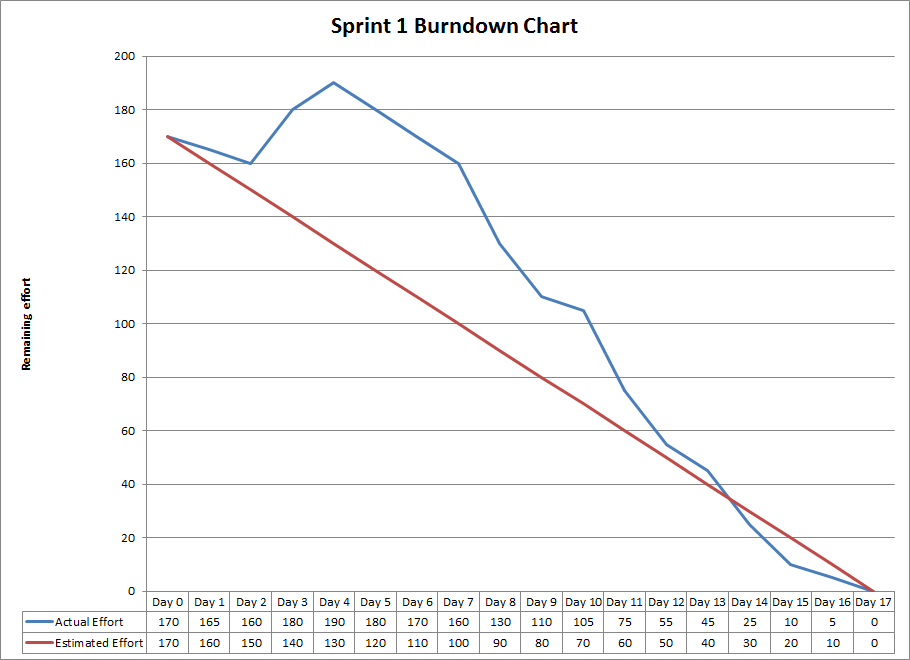
\includegraphics[width=1.0\textwidth]{images/burndown}
\end{center}\end{figure}

\pagebreak

\section{Individual Retrospective}
Actions to \textbf{start} doing (top 3)
\begin{itemize}
\item Run the accessibility linter in CI, not just before demos.
\item Mock the geocoding API in tests to avoid rate-limit flakiness.
\item Write API contract tests before wiring the frontend.
\end{itemize}
Actions to \textbf{stop} doing (top 3)
\begin{itemize}
\item Hardcoding category lists instead of loading them from config.
\item Committing secrets to the repo (moved to the secrets manager).
\item Skipping mobile-width checks until the end.
\end{itemize}
Actions to \textbf{continue} doing (top 3)
\begin{itemize}
\item Pairing on the API contract with John.
\item Keeping integrations behind adapters (swap-friendly).
\item Short daily blocker syncs.
\end{itemize}

\section{Peer Review}
Candid individual assessment; not shared. Each item graded 1--5. \\
Evaluation items:
\begin{itemize}
\item \textbf{Participation} - present and contributing?
\item \textbf{Communication} - timely, effective updates?
\item \textbf{Work quality} - claimed tasks; met objectives; added value?
\item \textbf{Professionalism} - professional and collaborative?
\item \textbf{Overall} - overall value this period.
\end{itemize}
\begin{tabular}{| p{1.5in} | >{\centering\arraybackslash} p{1.in} | >{\centering\arraybackslash} p{1.1in} | >{\centering\arraybackslash} p{1.1in}| >{\centering\arraybackslash} p{0.5in}| >{\centering\arraybackslash} p{.5in} |}
\hline
\textbf{Team member name} & \textbf{Participation} & \textbf{Communication} & \textbf{Work quality} & \textbf{Professionalism} & \textbf{Overall} \\ \hline
Grace Hopper & 5 & 5 & 5 & 5 & 5\\ \hline
Alan Turing & 5 & 5 & 4 & 5 & 5\\ \hline
John Von Neumann & 5 & 4 & 5 & 5 & 5\\ \hline
Ada Lovelace & 4 & 5 & 5 & 4 & 5\\ \hline
Charles Babbage & 4 & 4 & 4 & 4 & 4\\ \hline
\end{tabular}
\end{document}
